%% Ein einfaches Template für einen Übungsbericht unter Verwendung des Hagenberg
%% Setups, basierend auf der LaTeX 'report' Standardklasse.
%%% äöüÄÖÜß  <-- keine deutschen Umlaute hier? UTF-faehigen Editor verwenden!

%%% Magic Comments zum Setzen der korrekten Parameter in kompatiblen IDEs
% !TeX encoding = utf8
% !TeX program = pdflatex
% !TeX spellcheck = de_DE
% !BIB program = biber

\documentclass[german,notitlepage,smartquotes]{hgbreport}
% Zulässige Optionen in [..]:
%    Hauptsprache: 'german' (default), 'english'
%    Option zur Umwandlung in typografische Anführungszeichen: 'smartquotes'
%    APA Zitierstil: 'apa'
%    Erzeuge keine separate Titelseite: 'notitlepage'
%%%-----------------------------------------------------------------------------

\RequirePackage[utf8]{inputenc} % bei Verw. von lualatex oder xelatex entfernen!

\renewcommand{\chapter}[1]{} % Deaktiviere den \chapter Befehl
\graphicspath{{images/}}     % Verzeichnis mit Bildern und Grafiken
\bibliography{references}    % Biblatex-Literaturdatei (references.bib)
\ExecuteBibliographyOptions{backref=false} % Keine Rückreferenzen bei Quellen

%%%-----------------------------------------------------------------------------
\setcounter{chapter}{3}	% <----- Auf die Übungsnummer setzen
%%%-----------------------------------------------------------------------------

\author{Julian Jany}                        % Name
\title{GP2 Generative Programmierung -- SS 2022\\ % Name der Übung
				Übungsabgabe \arabic{chapter}}
\date{\today}

%%%-----------------------------------------------------------------------------
\begin{document}
%%%-----------------------------------------------------------------------------
\maketitle
%%%-----------------------------------------------------------------------------

\lstset{language=[sharp]C,
		basicstyle=\ttfamily\footnotesize,
		keywordstyle=\color{blue}\ttfamily,
		stringstyle=\color{red}\ttfamily,
		commentstyle=\color[rgb]{0,0.608,0.333}\ttfamily, % ForestGreen
		morecomment=[l][\color{magenta}]{\#}
}
\lstset{language=XML,
		basicstyle=\ttfamily\footnotesize,
		keywordstyle=\color{blue}\ttfamily,
		stringstyle=\color{red}\ttfamily,
		commentstyle=\color[rgb]{0,0.608,0.333}\ttfamily,
		morecomment=[l][\color{magenta}]{\#}
}

%%%-----------------------------------------------------------------------------

\section{One, to generate them all}

\subsection{Lösungsidee}

Das \texttt{Model.xml} wird mittels von .NET bereitgestellten Methoden geparst und in einen "Xml-Objektgraphen" transformiert. 
Dieser Graph wird "depth-first" iteriert; dabei werden die Xml-Knoten/Elemente in ihre entsprechenden Sourcecode-Teile übersetzt.
Über die Properties einer Klasse muss zweimal iteriert werden, um die Deklarationen der Properties und die ToString-Methode der Klasse generieren zu können.

\subsection{Code}

\lstinputlisting[caption=Model.xml, language={XML}]{src/ClassGenerator/Model.xml}
\clearpage
\lstinputlisting[caption=ClassGenerator.tt, language={[sharp]C}]{src/ClassGenerator/ClassGenerator.tt}
\lstinputlisting[caption=ClassGenerator.cs (generated), language={[sharp]C}]{src/ClassGenerator/ClassGenerator.cs}
\lstinputlisting[caption=Program.cs, language={[sharp]C}]{src/ClassGenerator/Program.cs}

\clearpage

\subsection{Test}

\begin{figure}[h]
\centering
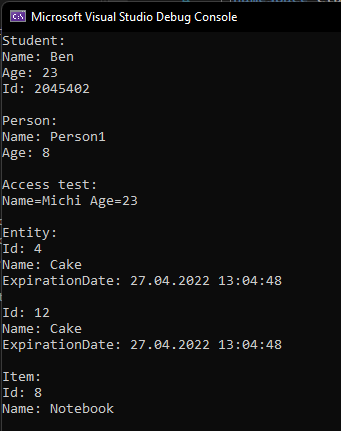
\includegraphics[width=.5\textwidth]{class_gen_test}
\caption{Testausgabe des ClassGenerator Projekts}
\label{fig:class_gen_test}
\end{figure}

%%%-----------------------------------------------------------------------------

\clearpage

\section{Clone ‘Em All!}

\subsection{Lösungsidee}

Gemeinsam in der Übung implementiert.

\subsection{Code}

\lstinputlisting[caption=A.cs, language={[sharp]C}]{src/CloningGenerator/A.cs}
\lstinputlisting[caption=B.cs, language={[sharp]C}]{src/CloningGenerator/B.cs}
\lstinputlisting[caption=CloningGenerator.tt, language={[sharp]C}]{src/CloningGenerator/CloningGenerator.tt}
\lstinputlisting[caption=CloningGenerator.cs (generated), language={[sharp]C}]{src/CloningGenerator/CloningGenerator.cs}
\lstinputlisting[caption=Program.cs, language={[sharp]C}]{src/CloningGenerator/Program.cs}

\subsection{Test}

\begin{figure}[h]
\centering
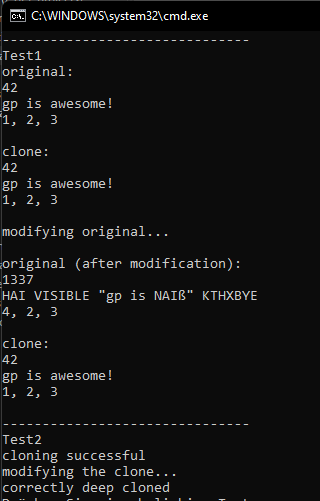
\includegraphics[width=.5\textwidth]{cloning_gen_test}
\caption{Testausgabe des CloningGenerator Projekts}
\label{fig:cloning_gen_test}
\end{figure}

%%%-----------------------------------------------------------------------------

\clearpage

\section{SVG Generator}

\subsection{Lösungsidee}

Für \texttt{Rectangles} und \texttt{Polylines} wurden die entsprechenden Generatoren, Shapes und Templates implementiert. Für die Implementierung der \texttt{Polyline} wurde zusätzlich die Klasse \texttt{Point2D} implementiert, welche Punkte in einem 2D-Koordinatensystem abbilden kann. Das Testen der Implementierung wurde so umgesetzt, dass eine \texttt{List} mit den auszuführenden Test-Mothoden erstellt wird; diese wird anschließend iteriert, die Test-Methode aufgerufen und das Ergebnis (SVG) im \texttt{outputs/} Ordner gespeichert.

\subsection{Code}

% generators
\lstinputlisting[caption=DiagramGenerator.java, language={Java}]{src/DiagramGenerator/src/main/java/gp/generators/DiagramGenerator.java}
\lstinputlisting[caption=PointGenerator.java, language={Java}]{src/DiagramGenerator/src/main/java/gp/generators/PointGenerator.java}
\lstinputlisting[caption=PolylineGenerator.java, language={Java}]{src/DiagramGenerator/src/main/java/gp/generators/PolylineGenerator.java}
\lstinputlisting[caption=RectangleGenerator.java, language={Java}]{src/DiagramGenerator/src/main/java/gp/generators/RectangleGenerator.java}

\lstinputlisting[caption=Diagram.java, language={Java}]{src/DiagramGenerator/src/main/java/gp/Diagram.java}

% freemarker templates
\lstinputlisting[caption=diagram.ftl, language={XML}]{src/DiagramGenerator/src/main/resources/templates/diagram.ftl}
\lstinputlisting[caption=point.ftl, language={XML}]{src/DiagramGenerator/src/main/resources/templates/point.ftl}
\lstinputlisting[caption=polyline.ftl, language={XML}]{src/DiagramGenerator/src/main/resources/templates/polyline.ftl}
\lstinputlisting[caption=rectangle.ftl, language={XML}]{src/DiagramGenerator/src/main/resources/templates/rectangle.ftl}

% shapes
\lstinputlisting[caption=Point2D.java, language={Java}]{src/DiagramGenerator/src/main/java/gp/shapes/helper/Point2D.java}
\lstinputlisting[caption=Point.java, language={Java}]{src/DiagramGenerator/src/main/java/gp/shapes/Point.java}
\lstinputlisting[caption=Polyline.java, language={Java}]{src/DiagramGenerator/src/main/java/gp/shapes/Polyline.java}
\lstinputlisting[caption=Rectangle.java, language={Java}]{src/DiagramGenerator/src/main/java/gp/shapes/Rectangle.java}

\lstinputlisting[caption=Test.java, language={Java}]{src/DiagramGenerator/src/main/java/gp/Test.java}
\lstinputlisting[caption=Main.java, language={Java}]{src/DiagramGenerator/src/main/java/gp/Main.java}

\clearpage

\subsection{Test}

\begin{figure}[h]
\centering
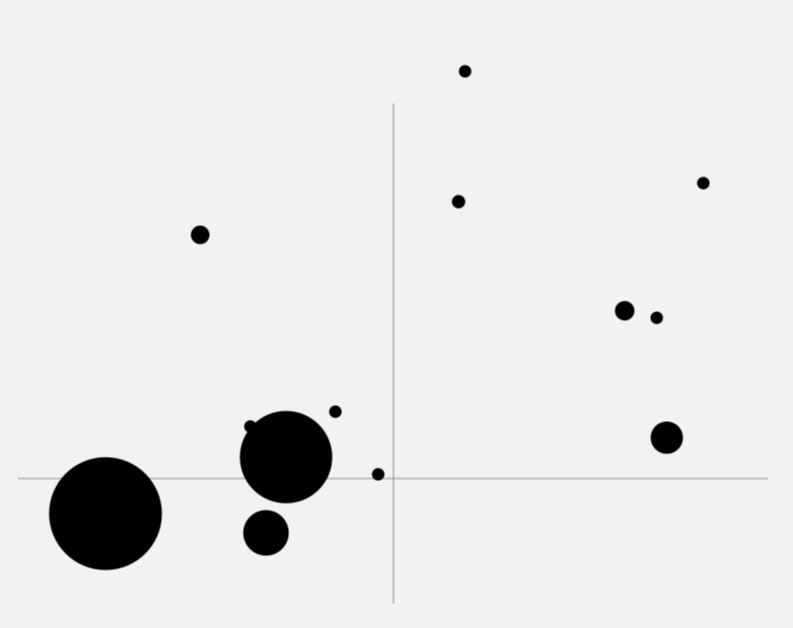
\includegraphics[width=.5\textwidth]{test-01}
\caption{Gerenderter SVG-Output von \texttt{createBubbleChart()}}
\label{fig:test-01}
\end{figure}

\begin{figure}
\centering
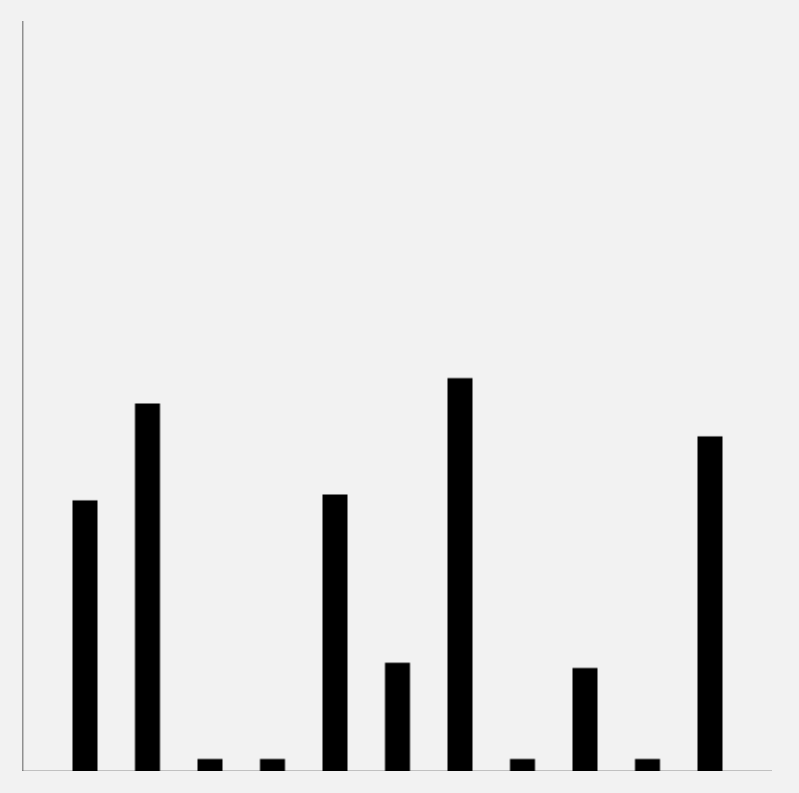
\includegraphics[width=.5\textwidth]{test-02}
\caption{Gerenderter SVG-Output von \texttt{createBarChart()}}
\label{fig:test-02}
\end{figure}

\begin{figure}
\centering
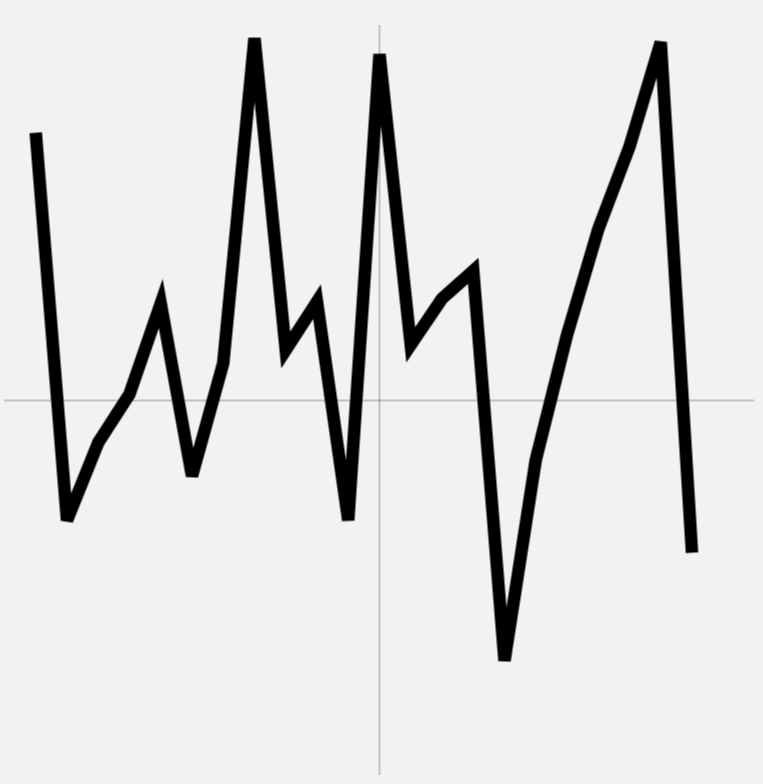
\includegraphics[width=.5\textwidth]{test-03}
\caption{Gerenderter SVG-Output von \texttt{createPoly()}}
\label{fig:test-03}
\end{figure}

\begin{figure}
\centering
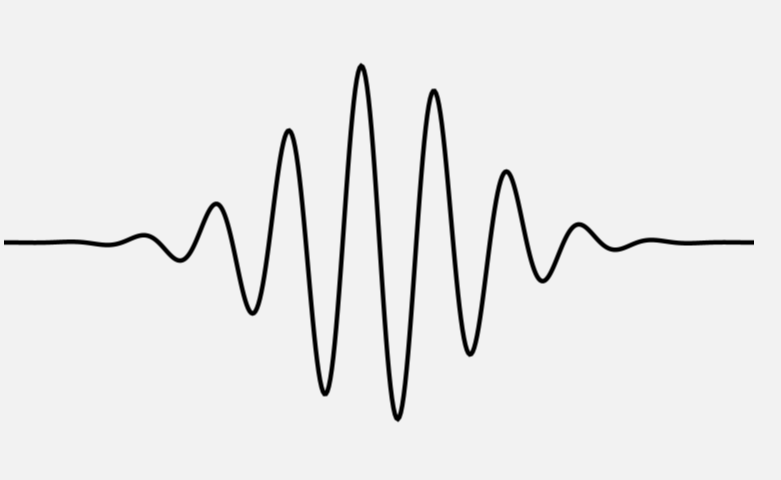
\includegraphics[width=.7\textwidth]{test-04}
\caption{Gerenderter SVG-Output von \texttt{createFunctionGraph()}}
\label{fig:test-04}
\end{figure}

\begin{figure}
\centering
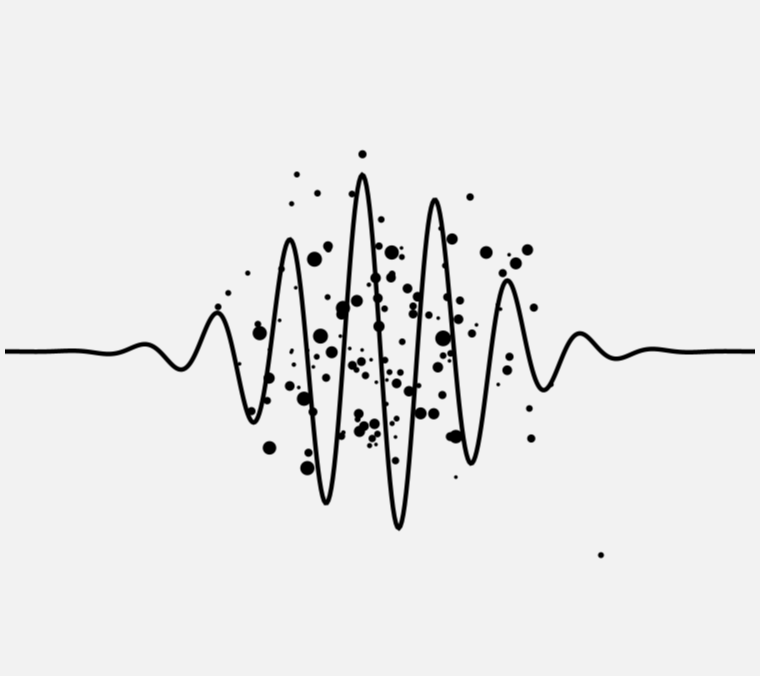
\includegraphics[width=.7\textwidth]{test-05}
\caption{Gerenderter SVG-Output von \texttt{createMultiple()}}
\label{fig:test-05}
\end{figure}

%%%-----------------------------------------------------------------------------

%\section*{Zusammenfassung und Anmerkungen}

%%%-----------------------------------------------------------------------------

% \section*{Quellen}

% \printbibliography[heading=noheader]

%%%-----------------------------------------------------------------------------
\end{document}
%%%-----------------------------------------------------------------------------